
\section{Ergebnisse und Diskussion}\label{chap:results}

In diesem Kapitel werden die Ergebnisse der einzelnen Zwischenschritte der Methodik nach \autoref{chap:Methodik} dargestellt und kritisch betrachtet.
Hierzu gehören vorerst die Ergebnisse der Clusterung der \gls{MS}-Netzgebiete, die mit \gls{SIMBEV} erzeugten Fahrtprofile und Standzeiten von \gls{EPKW} und deren räumlicher Verteilung, sowie die Ergebnisse der Implementierung der verschiedenen Ladestrategien.
Abschließend erfolgt eine detaillierte Betrachtung der Ergebnisse der Ermittlung des Abregelungsbedarfes aufgrund der Integration von \glspl{EPKW} für die untersuchten Netze.


\subsection{Erzeugung und Charakteristik der Fahrtprofile}

Mit Hilfe des Software Tools \gls{SIMBEV} werden für die Referenznetzgebiet die Fahrtprofile der im Netzgebiet befindlichen Fahrzeuge erstellt.
Die Charakteristik der Fahrtprofile spielt eine entscheidende Rolle für die Wirksamkeit der unterschiedlichen Ladestrategien und die Auswirkungen auf die Netze.
Hierbei steht vor allem die Jahresfahrleistung der \glspl{EPKW}, der Anteil flexibilisierbarer und nicht-flexibilisierer Ladevorgänge, die Gleichzeitigkeit der Ladevorgänge und wann diese auftreten im Vordergrund.
Innerhalb dieses Kapitels werden die Ergebnisse der Regionalisierung dargestellt, sowie die Charakteristik der erzeugten Fahrtprofile kritisch betrachtet.
Dabei liegt der Fokus auf der Überprüfung der Plausibilität der Fahrtprofile und dem herausstellen des Flexibilisierungspotentials von Ladevorgängen von \gls{EPKW}.\medskip

Die Ermittlung der Anzahl der Fahrzeuge erfolgt nach \autoref{chap:simbev_theo} auf Gemeindeebene.
In der Regel liegen innerhalb eines Netzgebietes mehrere Gemeinden und insgesamt liegen \num{35} Gemeinden innerhalb der sechs Referenznetzgebiete.
Die Auswertung ergibt die Anzahl der simulierten Fahrzeuge nach \autoref{tab:car_count} je Fahrzeugtyp und Szenario.
Zusätzlich findet sich im Anhang in \autoref{tab:car_count_long} eine detailliertere Aufteilung je Fahrzeugtyp, -klasse und Szenario.

{
\renewcommand{\arraystretch}{1.2}% grßerer Zeilenabstand
\sisetup{range-phrase=~{--}~}% Gedankenstrich statt "bis" bei SIrange
\begin{table}[H]
	\begin{center}
		\caption{Anzahl der Fahrzeuge in den Gemeinden der Referenznetzgebiete je Typ und Szenario}
		\begin{tabu} to 0.6\textwidth {X[1.2] X[1, r] X[1, r] X[1, r]}
			\toprule
			Szenario         & BEV         & PHEV        & Summe       \\ \midrule
			NEP C~\num{2035} & \num{14270} & \num{8841}  & \num{23111} \\
			Referenz         & \num{25545} & \num{15826} & \num{41371} \\
			Antriebswende    & \num{48617} & \num{30117} & \num{78734} \\ \bottomrule
		\end{tabu}
		\label{tab:car_count}
	\end{center}
	\vspace{-3mm}%Put here to reduce too much white space after your table
\end{table}
}

Die \num{35} Gemeinden weisen drei der sieben \gls{REGIOSTAR} (s. \autoref{tab:RegioStaR}) auf.
Hierzu zählen der kleinstädtische, dörfliche Raum einer ländlichen Region (\gls{ID} \num{77}), Mittelstädte im städtischen Raum (\gls{ID} \num{76}) und Mittelstädte im städtischen Raum einer Stadtregion (\gls{ID} \num{73}).
Die Jahresfahrleistung von \glspl{BEV} je \gls{REGIOSTAR} wurde zusammenfassend über alle Szenarien hinweg berechnet und findet sich in \autoref{tab:bev_distance}.
Dabei zeigt sich, dass in \gls{ID} \num{77} im Schnitt die weitesten Strecken zurückgelegt werden, welches den Erwartungen nach \gls{MID} \cite{Nobis2019} entspricht.
Jedoch liegen die Jahresfahrleistungen insgesamt unter den Angaben des \gls{MID} von durchschnittlich \SI{14700}{\km}, aber auf einem ähnlichen Niveau zu einer Auswertung von Kfz-Versicherungen des Vergleichsportals \textit{Check24} \cite{CHECK24GmbH2018}, wonach die durchschnittliche Jahresfahrleistung in Deutschland im Jahr \num{2017} bei \SI{11888}{\km} lag.
Insgesamt spiegeln die Jahresfahrleistungen \glspl{SIMBEV} somit ein progressives Szenario mit einer sinkenden Jahresfahrleistung wider.


{
\renewcommand{\arraystretch}{1.2}% grßerer Zeilenabstand
\sisetup{range-phrase=~{--}~}% Gedankenstrich statt "bis" bei SIrange
\begin{table}[H]
	\begin{center}
		\caption{Durchschnittliche Jahresfahrleistung mit Standardabweichung und maximale Jahresfahrleistung von BEVs je untersuchter RegioStaR 7 Raumtypologie}
		\begin{tabu} to 0.8\textwidth {X[0.2] X[1.6, r] X[1.5, r]}
			\toprule
			ID 	   				   & Durchschnittle Jahresfahrleistung                  & Maximale Jahresfahrleistung \\ \midrule
			\num{73}               & \SI[separate-uncertainty = true]{11660(6408)}{\km} & \SI{58575}{\km}             \\
			\num{76}               & \SI[separate-uncertainty = true]{11500(6243)}{\km} & \SI{54204}{\km}             \\
			\num{77}               & \SI[separate-uncertainty = true]{12353(6395)}{\km} & \SI{55426}{\km}             \\ \bottomrule
		\end{tabu}
		\label{tab:bev_distance}
	\end{center}
	\vspace{-3mm}%Put here to reduce too much white space after your table
\end{table}
}

Eine Betrachtung der durchschnittlichen Stand- und Ladezeiten von Ladevorgängen bei maximal möglicher Ladeleistung der \gls{EPKW} je Wegezweck in \autoref{tab:StandingTime} zeigt, dass die \gls{EPKW} vor allem im privaten Bereich einen Großteil der Standzeit nicht geladen werden.
So macht die durchschnittliche Ladezeit der Wegezwecke \nH und \Arbeit nur etwa \SI{8}{\percent} der Standzeit aus.
Hierbei sind zwar auch Fahrten enthalten, die im öffentlichen Raum am Straßenrand enden, dennoch zeigt sich deutlich das große Flexibilisierungspotential im privaten Bereich.
% Da Ladevorgänge im öffentlichen Raum erst ab einem \gls{SOC} von \SI{80}{\percent} ausgelöst werden, liegt die Ladezeit der sonstigen Wegezwecke über den Wegezwecken \nH und \Arbeitdot.
% Allerdings zeigt sich auch hier, dass in den meisten Fällen ein großes Flexibilisierungspotential vorliegt.
% Es empfiehlt sich somit auch die Wirksamkeit von netzdienlichen Ladestrategien im öffentlichen Raum zu untersuchen, welches nicht in dieser Arbeit behandelt wird.

{
\renewcommand{\arraystretch}{1.2}% grßerer Zeilenabstand
\sisetup{range-phrase=~{--}~}% Gedankenstrich statt "bis" bei SIrange
\begin{table}[H]
	\begin{center}
		\caption{Durchschnittliche Stand- und Ladezeiten von Ladevorgängen je Wegezweck mit Standardabweichung}
		\begin{tabu} to 0.8\textwidth {X[0.5] X[1, r] X[1, r]}
			\toprule
			Wegezweck  & Durchschnittliche Standzeit                      & Durchschnittliche Ladezeit	                     \\ \midrule
			Arbeit     & \SI[separate-uncertainty = true]{7.3(37)}{\hour} & \SI[separate-uncertainty = true]{0.6(5)}{\hour}  \\
%			dienstlich & \SI[separate-uncertainty = true]{4.4(58)}{\hour} & \SI[separate-uncertainty = true]{1.1(7)}{\hour}  \\
%			Ausbildung & \SI[separate-uncertainty = true]{6.2(39)}{\hour} & \SI[separate-uncertainty = true]{1.4(11)}{\hour} \\
%			Einkauf    & \SI[separate-uncertainty = true]{2.1(38)}{\hour} & \SI[separate-uncertainty = true]{0.8(5)}{\hour}  \\
%			Erledigung & \SI[separate-uncertainty = true]{4.2(56)}{\hour} & \SI[separate-uncertainty = true]{0.9(6)}{\hour}  \\
%			Freizeit   & \SI[separate-uncertainty = true]{6.0(62)}{\hour} & \SI[separate-uncertainty = true]{1.1(7)}{\hour}  \\
			nach Hause & \SI[separate-uncertainty = true]{8.9(57)}{\hour} & \SI[separate-uncertainty = true]{0.7(6)}{\hour}  \\ \bottomrule
		\end{tabu}
		\label{tab:StandingTime}
	\end{center}
	\vspace{-3mm}%Put here to reduce too much white space after your table
\end{table}
}

Der Anteil flexibilisierbarer Ladevorgänge entspricht dem Anteil an Energie am Gesamtenergiebedarf der \glspl{EPKW}, der an privaten Ladepunkten zu Hause oder an Firmenparkplätzen nachgeladen wird.
Hierzu zählen alle Ladevorgänge die am Eigenheim, einer Wohnanlage oder auf einem Firmenparkplatz stattfinden.
Zusätzlich sind nur Ladevorgänge flexibilisierbar, deren Standzeit größer ist als die Mindestladedauer.
Demgegenüber stehen nicht-flexibilisierbare Ladevorgänge im öffentlichen Raum und an Schnellladestationen bzw. Ladevorgänge deren Standzeit der Mindestladedauer entspricht.
Im Mittel liegt der Anteil flexibilisierbarer Ladevorgänge über alle Szenarien je Gemeinde bei \SI{71.1}{\percent}.
Hiervon ausgenommen ist die \SzeFirmenparkplatzdot, bei der es aufgrund des geringeren Bestands an Ladeinfrastruktur an Firmenparkplätzen zu mehr Ladevorgängen im öffentlichen Raum kommt.
Der Anteil flexibilisierbarer Ladevorgänge liegt bei dieser Szenarette bei \SI{66.1}{\percent}.
In \autoref{tab:ChargingShare} sind die Anteile flexibilisierbarer und nicht-flexibilisierbarer Ladevorgänge zusammengefasst.

{
\renewcommand{\arraystretch}{1.2}% grßerer Zeilenabstand
\sisetup{range-phrase=~{--}~}% Gedankenstrich statt "bis" bei SIrange
\begin{table}[H]
	\begin{center}
		\caption{Aufteilung in flexibiliserbare und nicht-flexibiliserbare Ladevorgänge nach dem Anteil vom Gesamtenergiebedarf der E-Pkw je Gemeinde mit Standardabweichung}
		\begin{tabu} to 0.9\textwidth {X[1] X[1.3, r] X[1, r]}
			\toprule
								  					& \SzeFirmenparkplatzdot                               & Sonstige Szenarien                                   \\ \midrule
			Flexibilisierbar       	& \SI[separate-uncertainty = true]{66.1(23)}{\percent} & \SI[separate-uncertainty = true]{71.1(23)}{\percent} \\
			Nicht-flexibilisierbar 	& \SI[separate-uncertainty = true]{33.9(23)}{\percent} & \SI[separate-uncertainty = true]{28.9(23)}{\percent} \\ \bottomrule
		\end{tabu}
		\label{tab:ChargingShare}
	\end{center}
	\vspace{-3mm}%Put here to reduce too much white space after your table
\end{table}
}

In \autoref{fig:example_load_profile} findet sich beispielhaft das \gls{EPKW}-Lastprofil für Referenz-Laden des Netzgebietes \num{176} über eine Woche im Antriebswende-Szenario (links).
Zusätzlich ist das \gls{EPKW}-Lastprofil der gleichen Gemeinde in der \SzeFirmenparkplatz (rechts) dargestellt.

\begin{figure}[H]
    \centering
    \includegraphics[width=\textwidth]{Bilder/example_load_profile}
    \caption[E-Pkw-Lastprofil für Referenz-Laden im Netz \num{176} der simulierten Woche im Antriebswende-Szenario und der Sensitivität Firmenparkplatz]{E-Pkw-Lastprofil (netzseitige Last; inkl. Umwandlungsverluste) für Referenz-Laden im Netz \(176_{\text{PV}}\) der simulierten Woche im Antriebswende-Szenario (links) und der \SzeFirmenparkplatz (rechts)}\label{fig:example_load_profile}
\end{figure} % TODO: Leistung statt Last

Die Lastgänge \zH und \Firmeparkplatz entsprechen den Ladevorgängen im privaten Bereich.
Unter dem Lastgang \oeffen sind hingegen alle öffentlichen Ladevorgänge mit Ausnahme der Schnellladevorgänge (\gls{HPC}) zusammengefasst.
Deutlich zu erkennen ist die hohe Gleichzeitigkeit am Vormittag sowohl an Firmenparkplätzen als auch im öffentlichen Raum, welche durch das Fahren zur Arbeit ausgelöst wird.
Auch die Rückkehr zum Wohnort ist ab dem frühen Nachmittag in den Lastgängen \zH und im öffentlichen Raum deutlich zu erkennen.
Schnellladevorgänge treten unregelmäßig im Verlauf der Woche auf.
Vor allem am Sonntag kommt es zu deutlich geringeren Anteilen von Ladevorgängen zu Hause und am Firmenparkplatz, wodurch das Flexibilisierungspotential am Wochenende geringer ausfällt.
Gegenüber dem Antriebswende-Szenario sinkt die Höchstlast in der \SzeFirmenparkplatzdot, jedoch sinkt auch das Flexibilisierungspotential bei einem annähernd gleichbleibendem Energiebedarf durch die Verschiebung der Ladevorgänge in den öffentlichen Raum.\medskip
% TODO: erwähnen, dass durch die anderen Wahrscheinlichkeiten und dem Simulieren von nur einer Woche hier leichte Differenzen auftreten und auf Steckbriefe verweisen

Die entsprechenden Dauerlastkurven für die Gemeinde über eine Woche (s. \autoref{fig:example_load_curve}) zeigen nochmals deutlich die dominante Rolle der Hochlastphase die Aufgrund der hohen Gleichzeitigkeit des Wegezwecks \Arbeit vor allem am Firmenparkplatz aber auch im öffentlichen Raum auftritt.
So wird im Antriebswende-Szenario eine Spitzenlast von \SI{14.8}{\mw} erreicht.
Im Netzgebiet \num{176} befinden sich im Antriebswende-Szenario \SI{26359}{\FZ}, welches einem Verhältnis von Spitzenlast zu Fahrzeugen von \SI{0.56}{\kWperFZ} entspricht.
Zum Vergleich wurde in der \textit{Kurzstudie Elektromobilität} für den \gls{NEP} \cite{Ebner2019} für \SI{12}{\MioStk} innerhalb eines Jahres eine Spitzenlast von \SI{12}{\gw} ermittelt, welches einem Verhältnis von \SI{1.00}{\kWperFZ} entspricht.
Für eine mittlere Woche liegt die Spitzenlast in der \textit{Kurzstudie Elektromobilität} bei \SI{9}{\gw} und somit bei \SI{0.75}{\kWperFZ}.
Die Spitzenlast wird nach der \textit{Kurzstudie Elektromobilität} in der Regel am Nachmittag erreicht, da im Vergleich zu dieser Arbeit deutlich weniger Ladevorgänge an Firmenparkplätzen stattfinden.
Hierdurch ergibt sich innerhalb der Woche am Abend eine besonders hohe Gleichzeitigkeit beim Laden \zHdot, während in der durchgeführten Simulation dieser Arbeit täglich zwei Leistungsspitzen mit einer geringeren Gleichzeitigkeit am Morgen und am Nachmittag auftreten.
Das Ergebnis liegt somit in einer ähnlichen Dimension und die Ergebnisse der Simulation können als plausibel angesehen werden.

% TODO: CP E-Bedarf je grid id und Szenario



\begin{figure}[H]
    \centering
    \includegraphics[width=\textwidth]{Bilder/example_load_duration_curve}
    \caption[E-Pkw-Dauerlastkurve für Referenz-Laden im Netz \num{176} über eine Woche im Antriebswende-Szenario und der Sensitivität Firmenparkplatz]{E-Pkw-Dauerlastkurve (netzseitige Last; inkl. Umwandlungsverluste) für Referenz-Laden im Netz \(176_{\text{PV}}\) über eine Woche im Antriebswende-Szenario (oben) und der \SzeFirmenparkplatz (unten)}\label{fig:example_load_curve}
\end{figure} % TODO: Leistung statt Last

Zum Zeitpunkt der Erstellung der Fahrtprofile war es noch nicht möglich, einen längeren Zeitraum als eine Woche am Stück zu simulieren.
Durch die Zuordnung eines zufälligen Eingangs-\gls{SOC} für einige Fahrzeuge (s. \autoref{chap:simbev_theo}) fällt der Ladebedarf am Montag nicht deutlich aus der Reihe.
Jedoch kann hierdurch ein weiterer Effekt nitch verhindert werden.
Bei Fahrzeugen, welche weder einen festen Ladepunkt zu Hause oder an Firmenparplätzen zugewiesen bekommen haben, fällt der \gls{SOC} im Laufe der Woche langsam ab.
Hierdurch kommt es durch die Abhängigkeit der Ladewahrscheinlichkeit vom \gls{SOC} zu einer Zunahme des Ladebedarfs im öffentlichen Raum über die Woche.
Es ist zu vermuten, dass dies weiterhin dazu führt, dass Ladevorgänge an Schnellladeinfrastruktur un­ter­re­prä­sen­tiert dargestellt werden.


\subsection{Verteilung der Ladevorgänge auf die Ladeinfrastruktur}\label{chap:distribute_demand_ev}

Die Verteilung der Ladevorgänge auf eine konkrete georeferenzierte Ladeinfrastruktur nach \autoref{chap:theo_distribution} liefert je Netzgebiet eine Vielzahl von unterschiedlichen Netzanschlusspunkten.
In \autoref{fig:cps_in_grid} finden sich beispielhaft die ermittelten Netzanschlusspunkte für Ladeinfrastruktur innerhalb des Netzgebietes \num{176} für das Antriebswende-Szenario für Ladeinfrastruktur zu Hause, an Firmenparkplätzen, Normalladeinfrastruktur im öffentlichen Raum und für Schnellladeinfrastruktur (\gls{HPC}).
Es wird deutlich, dass die Ladeinfrastruktur \zH die meisten Netzanschlusspunkte aufweist, während für die Schnellladeinfrastruktur nur wenige Netzanschlusspunkte benötigt werden.

\begin{figure}[H]
    \centering
    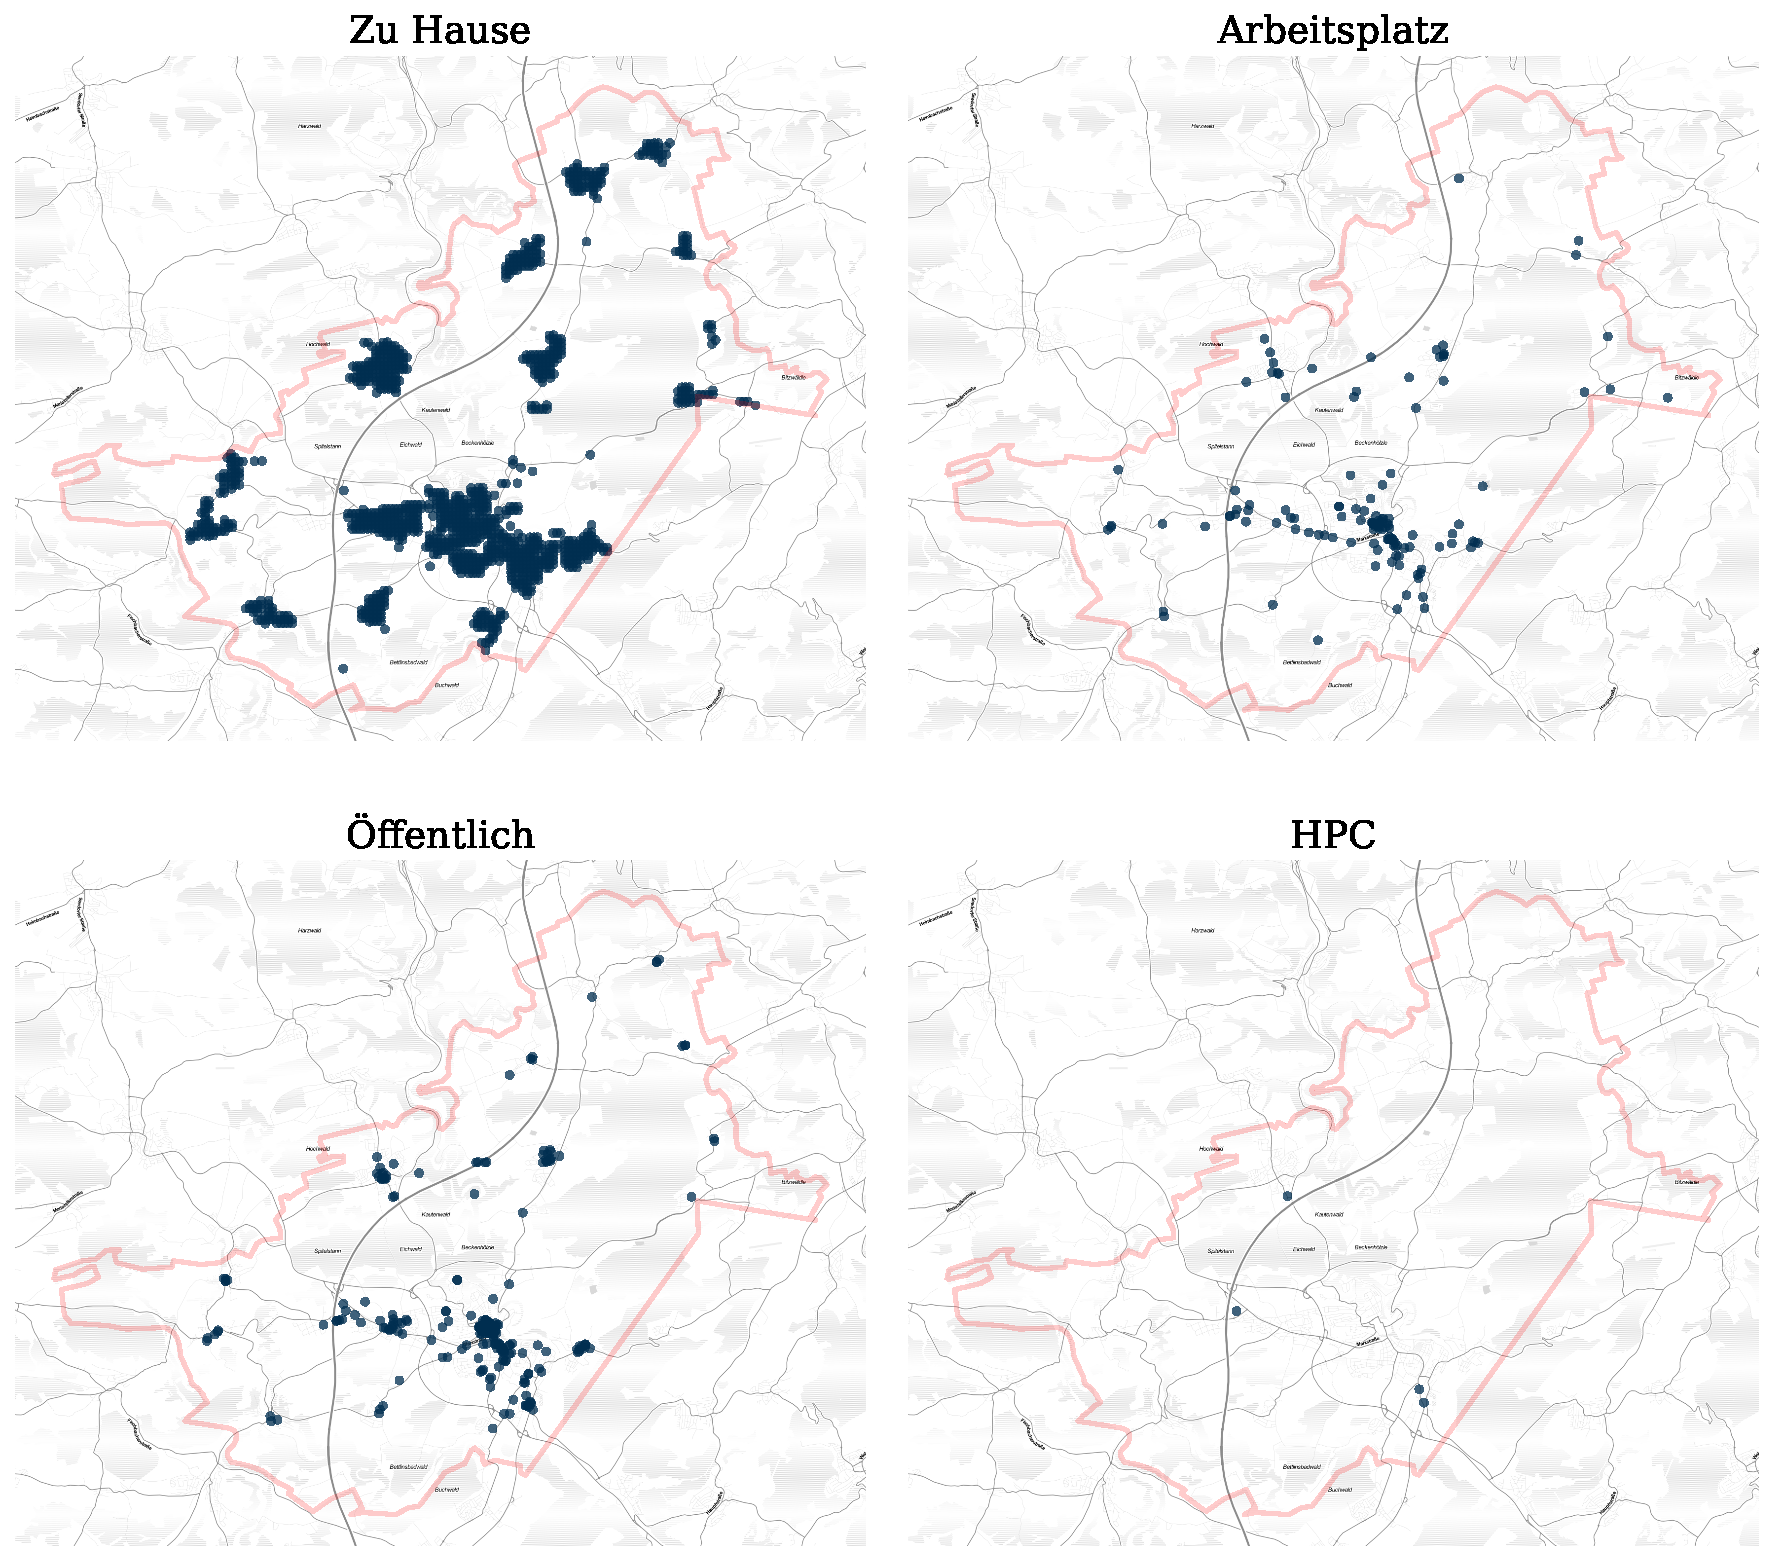
\includegraphics[width=\textwidth]{Bilder/cps_in_grid_176}
    \caption[Geographische Verteilung der ermittelten Netzanschlusspunkte für Ladeinfrastruktur im Netz \num{176} für das Antriebswende-Szenario je Lade Use Case]{Geographische Verteilung der ermittelten Netzanschlusspunkte für Ladeinfrastruktur im Netz \(176_{\text{PV}}\) für das Antriebswende-Szenario je Lade Use Case}\label{fig:cps_in_grid}
\end{figure}

Neben der geographischen Lokalisation der Ladeinfrastruktur ist es für die Netzuntersuchungen entscheidend, ob die Ladeinfrastruktur in der \gls{NS}- oder \gls{MS}-Ebene angeschlossen ist.
Wenn der Anschluss in der \gls{NS}-Ebene erfolgt, dann werden sowohl die Betriebsmittel der \gls{MS}- und \gls{MS}-Ebene belastet, während bei einem Anschluss in der \gls{MS}-Ebene auch nur diese betroffen ist.
Außerdem findet ab einem Anschluss von privater Ladeinfrastruktur in der \gls{MS}-Ebene auch bei der Referenz-Ladestrategie reduziertes Laden statt (s. \autoref{chap:theo_strategies}).
In \autoref{tab:lvConnectionShare} findet sich der Anteil des in der \gls{NS}-Ebene anfallenden Energiebedarfs vom Gesamtenergiebedarf der Ladeinfrastruktur im Netzgebiet.
Es wird deutlich, dass der Anteil von Ladeinfrastruktur in der \gls{MS}-Ebene mit einer steigenden Zahl von Fahrzeugen zunimmt.
Gleichzeitig zeigt sich, dass in der \SzeFirmenparkplatz der Anteil von Ladeinfrastruktur in der \gls{MS}-Ebene deutlich geringer ausfällt als im Antriebswende-Szenario, trotz einer gleichen Anzahl an \gls{EPKW} innerhalb der Szenarien.
Dies lässt sich damit erklären, dass neben der öffentlichen Ladeinfrastruktur vor allem Ladeinfrastruktur auf Firmenparkplätzen einen Anschluss in der \gls{MS}-Ebene benötigt.
Da im Antriebswende-Szenario mehr Ladepunkte auf eine gleichbleibende Anzahl von möglichen Anschlusspunkten für Ladeinfrastruktur auf Firmenparkplätzen verteilt werden müssen, fällt die Anschlussleistung dieser Ladeinfrastruktur deutlich höher aus und macht somit einen Anschluss in der \gls{MS}-Ebene nötig.

{
\renewcommand{\arraystretch}{1.2}% grßerer Zeilenabstand
\sisetup{range-phrase=~{--}~}% Gedankenstrich statt "bis" bei SIrange
\begin{table}[H]
	\begin{center}
		\caption{Anteil des in der NS-Ebene anfallenden Energiebedarfs vom Gesamtenergiebedarf der Ladeinfrastruktur je Szenario}
		\begin{tabu} to \textwidth {X[0.5] X[1, r] X[1, r] X[1.2, r] X[1.2, r]}
			\hline
			Netz ID    & NEP C \num{2035}    & Referenz            & Antriebswende       & \glqq Firmenparkplatz\grqq \\ \hline
			\num{176}  & \SI{98.0}{\percent} & \SI{92.9}{\percent} & \SI{82.0}{\percent} & \SI{91.3}{\percent}        \\
			\num{177}  & \SI{96.6}{\percent} & \SI{86.8}{\percent} & \SI{77.8}{\percent} & \SI{86.7}{\percent}        \\
			\num{1056} & \SI{99.8}{\percent} & \SI{99.5}{\percent} & \SI{94.0}{\percent} & \SI{97.9}{\percent}        \\
			\num{1690} & \SI{99.8}{\percent} & \SI{97.0}{\percent} & \SI{86.5}{\percent} & \SI{92.9}{\percent}        \\
			\num{1811} & \SI{99.9}{\percent} & \SI{98.7}{\percent} & \SI{90.0}{\percent} & \SI{95.2}{\percent}        \\
			\num{2534} & \SI{99.7}{\percent} & \SI{97.4}{\percent} & \SI{80.8}{\percent} & \SI{91.4}{\percent}        \\ \hline
		\end{tabu}
		\label{tab:lvConnectionShare}
	\end{center}
	\vspace{-3mm}%Put here to reduce too much white space after your table
\end{table}
}


In \autoref{tab:largestLVGridShare} ist die Anzahl an \gls{NS}-Netzen je \gls{MS}-Netzgebiet und der maximal anfallender Energieanteil eines \gls{NS}-Netzes am Gesamtenergiebedarf der Ladeinfrastruktur in der \gls{NS}-Ebene in allen betrachteten Szenarien dargestellt.
Hierbei wird deutlich, dass es in einigen \gls{MS}-Netzgebieten zu einer starken lokalen Konzentration an Ladeinfrastruktur kommt.
So entfallen beispielsweise im \gls{MS}-Netzgebiet \num{2534} im NEP C~\num{2035} Szenario \SI{62.3}{\percent} des Energiebedarfs der Ladeinfrastruktur in der \gls{NS}-Ebene innerhalb eines einzigen \gls{NS}-Netzes an.
Auch im \gls{MS}-Netzgebiet \num{176} zeigt sich eine starke lokale Konzentration innerhalb eines \gls{NS}-Netzes, welches sich in \autoref{fig:cps_in_grid} durch eine starke Konzentration der Ladeinfrastruktur in den bewohnten Regionen widerspiegelt.
In der Realität würde es bei solch starken lokalen Konzentrationen vermutlich zu einem Netzneubau kommen, welcher innerhalb dieser Arbeit nicht abgebildet werden kann.

{
\renewcommand{\arraystretch}{1.2}% grßerer Zeilenabstand
\sisetup{range-phrase=~{--}~}% Gedankenstrich statt "bis" bei SIrange
\begin{table}[H]
	\begin{center}
		\caption{Anzahl der NS-Netze je MS-Netzgebiet und maximal anfallender Energieanteil eines NS-Netzes am Gesamtenergiebedarf der Ladeinfrastruktur in den NS-Netzen mit Standardabweichung je MS-Netzgebiet und Szenario}
		\begin{tabu} to 0.8\textwidth {X[0.5] X[1, r] X[2, r]}
			\hline
			Netz ID    & Anzahl NS-Netze & Maximaler Ladeanteil eines NS-Netzes                 \\ \hline
			\num{176}  & \num{105}       & \SI[separate-uncertainty = true]{34.7(12)}{\percent} \\
			\num{177}  & \num{56}        & \SI[separate-uncertainty = true]{25.5(8)}{\percent}  \\
			\num{1056} & \num{130}       & \SI[separate-uncertainty = true]{12.3(7)}{\percent}  \\
			\num{1690} & \num{179}       & \SI[separate-uncertainty = true]{11.2(1)}{\percent}  \\
			\num{1811} & \num{381}       & \SI[separate-uncertainty = true]{7.4(3)}{\percent}   \\
			\num{2534} & \num{9}         & \SI[separate-uncertainty = true]{61.1(7)}{\percent}  \\ \hline
		\end{tabu}
		\label{tab:largestLVGridShare}
	\end{center}
	\vspace{-3mm}%Put here to reduce too much white space after your table
\end{table}
}


\subsection{Ergebnisse der Implementierung der Ladestrategien}\label{chap:results_charging_strategies}

Im Rahmen der Netzuntersuchungen kommt den Zeitreihen der Last der \glspl{EPKW} die größte Bedeutung zu, da die Last und Erzeugung aller anderen Verbraucher und Erzeuger nicht veränderlich ist.
Das Ziel der Ladestrategien (s. \autoref{chap:theo_strategies}) ist es, die Netzbelastung möglichst gering zu halten.
Bei den Ladegruppen und reduzierten Laden soll dies durch ein präventives Lademanagement und bei dem Residuallast-Laden durch ein aktives Lademanagement erreicht werden.

\begin{figure}[H]
    \centering
    \includegraphics[width=1\textwidth]{Bilder/example_resiual_load}
    \caption[Residuallast über ein Jahr im Netz \num{176} für das Antriebswende-Szenario]{Residuallast über ein Jahr im Netz \(176_{\text{PV}}\) für das Antriebswende-Szenario}\label{fig:residual_load}
\end{figure}

\autoref{fig:residual_load} zeigt beispielhaft für das Netzgebiet \num{176} die Abhängigkeit der Residuallast von der Ladestrategie im Antriebswende-Szenario.
Dabei zeigt sich, dass vor allem die Residuallast-Ladestrategie zu einer klaren Glättung der Residuallastkurve führt, während sich bei den sonstigen Ladestrategien ein ähnliches Bild zeigt.
Dabei führen die Ladegruppen gegenüber dem Referenz-Laden sogar zu einem gegensätzlichen Effekt und zu einer Erhöhung der Spitzenlast im Last- und Rückspeisefall.
In \autoref{fig:residual_load_diff} ist die Veränderung der Residuallast über ein Jahr in Abhängigkeit von den verschiedenen Ladestrategien dargestellt.
Dabei zeigt die Darstellung der Referenz-Ladestrategie (oben links) die Residuallast über ein Jahr, während in den anderen drei Darstellungen die Differenz der jeweiligen Ladestrategie zum Referenz-Laden abgebildet wird.
Bei den Ladegruppen zeigt sich gegenüber dem Referenz-Laden eine deutlich stärkere Belastung am Vormittag und ein Abfallen der Belastung bis zum Mittag.
Am Nachmittag lässt sich in der Regel keine Differenz feststellen.
Bei der reduzierten Ladestrategie kommt es zu einer leicht reduzierten Residuallast im Verlauf des Tages, während die Residuallast Nachts leicht zunimmt.
Die stärksten Veränderungen werden bei der Residuallast-Ladestrategie festgestellt.
Da es sich bei dem Netzgebiet \num{176} um ein \gls{PV}-dominiertes Netz handelt, kommt es zu einer starken Verschiebung der Ladevorgänge in die Mittagszeit.
Auch kommt es zu einer deutlichen Verschiebung der Last in die Schwachlastzeit nach Mitternacht, während die Residuallast am Vor- und Nachmittag abnimmt.
Da auf diese weise jedoch nur Aussagen über das komplette \gls{MS}-Netzgebiet getroffen werden können, kann hier draus noch keine Aussage über die Belastung der einzelnen Betriebsmittel getroffen werden.

\begin{figure}[H]
    \centering
    \includegraphics[width=\textwidth]{Bilder/residual_load_diff}
    \caption{Veränderung des durchschnittlichen stündlichen Leistungsbedarfs von E-Pkw je Wochentag im Netz \num{176} für das Antriebswende-Szenario über ein Jahr in Abhängigkeit von der Ladestrategie}\label{fig:residual_load_diff}
\end{figure}

% TODO: Eventuell Auswertung, wie sich die Residuallast durch das Residuallast-Laden verändert bei den unterschiedlichen Netzgebieten und Szenarien
% TODO: Bubble maps


\subsection{Abregelungsbedarf innerhalb der untersuchten Netzgebiete}

In diesem Abschnitt werden die Ergebnisse der Ermittlung des Abregelungsbedarfs innerhalb der sechs untersuchten Netzgebiete dargestellt.
Dabei wird getrennt auf die drei Netz-Kategorien Last-, \gls{PV}- und Wind-dominiert eingegangen, um eine Aussage über die Wirksamkeit der Ladestrategien innerhalb der verschiedenen Netz-Kategorien treffen zu können.
Dabei werden die zwei Wochen mit der minimalen (kurz: Woche A) bzw. maximalen (kurz: Woche B) durchschnittliche Residuallast je Netz untersucht.
Die vollständigen Ergebnisse für die Ermittlung des Abregelungsbedarfs finden sich im Anhang in den Netz-Steckbriefen ab {\color{red} TODO}.


\subsubsection{Last-dominierte Netze}




\subsubsection{PV-dominierte Netze}

Die \gls{PV}-dominierten Netze \num{176} und \num{1056} besitzen stark unterschiedliche Charakteristika.
So weist das Netz \num{176} im Antriebswende-Szenario in der Woche A (minimale Residuallast) ein Verhältnis zwischen der Einspeisung von \glspl{FEE} und dem Ladebedarf der \glspl{EPKW} von etwa \(2:1\) auf, während dieses Verhältnis im Netz \num{1056} bei etwa \(11:1\) liegt.
Auch weist das Netz \num{176} eine deutlich größere Einspeisung von nicht-\gls{FEE} Anlagen auf und der Verbrauch der sonstigen Lasten ist mehr als dreimal so hoch als im Netz \num{1056}.
Eine Auflistung der wichtigsten Eckdaten für die Woche A beider Netze findet sich in \autoref{tab:pv_dominated_week_a_char}.

{
\renewcommand{\arraystretch}{1.2}% grßerer Zeilenabstand
\sisetup{range-phrase=~{--}~}% Gedankenstrich statt "bis" bei SIrange
\begin{table}[H]
	\begin{center}
		\caption{Einspeisung von fEE und nicht-fEE Anlagen sowie der Bedarf von sonstigen Lasten und E-Pkws je Szenario}
		\begin{tabu} to 0.7\textwidth {X[2] X[1, r] X[1, r]}
			\hline
													  & Netz \num{176}  & Netz \num{1056} \\ \hline
			Einspeisung fEE in \si{\mwh}              & \num{2262} & \num{4055} \\
			Einspeisung Sonstige in \si{\mwh}         & \num{1460} & \num{254}  \\
			Bedarf Sonstige  in \si{\mwh}             & \num{4197} & \num{1318} \\ \hline
			\multicolumn{3}{l}{Ladebedarf E-Pkw}                                \\ \hline
			NEP C~\num{2035} in \si{\mwh}             & \num{290}  & \num{109}  \\
			Referenz in \si{\mwh}                     & \num{520}  & \num{194}  \\
			Antriebswende in \si{\mwh}                & \num{988}  & \num{368}  \\
			\glqq Firmenparkplatz\grqq{} in \si{\mwh} & \num{974}  & \num{363}  \\ \hline
		\end{tabu}
		\label{tab:pv_dominated_week_a_char}
	\end{center}
	\vspace{-3mm}%Put here to reduce too much white space after your table
\end{table}
}

In {\color{red} TODO} findet sich der ermittelte Abregelungsbedarf für \glspl{FEE}, des Ladebedarfs und der sonstigen Lasten für die beiden Netze für die Referenz-Ladestrategie.
Es zeigt sich, dass der Abregelungsbedarf von \gls{FEE} Anlagen mit einem steigenden Anteil an \gls{EPKW} abnimmt und der Abregelungsbedarf aller Lasten zunimmt.
Hierbei fällt der Abregelungsbedarf von \gls{FEE} Anlagen in der \SzeFirmenparkplatz stärker ab als im Antriebswende-Szenario.
Dies lässt sich dadurch begründen, dass der Abregelungsbedarf des Ladebedarfs und von sonstigen Lasten in der \SzeFirmenparkplatz ebenfalls geringer ausfällt und somit ein besserer Ausgleich zwischen Angebot und Nachfrage erreicht werden kann.

{
\renewcommand{\arraystretch}{1.2}% grßerer Zeilenabstand
\sisetup{range-phrase=~{--}~}% Gedankenstrich statt "bis" bei SIrange
\begin{table}[H]
	\begin{center}
		\caption{Abregelungsbedarf von fEE Anlagen, sonstigen Lasten und E-Pkws je Szenario für die Referenz-Ladestrategie}
		\begin{tabu} to 0.7\textwidth {X[2] X[1, r] X[1, r]}
			\toprule
			Abregelung fEE							  & Netz \num{176} & Netz \num{1056} \\ \midrule
			NEP C~\num{2035} in \si{\mwh}             &                & \num{89}        \\
			Referenz in \si{\mwh}                     &                & \num{84}        \\
			Antriebswende in \si{\mwh}                &                & \num{76}        \\
			\glqq Firmenparkplatz\grqq{} in \si{\mwh} &                & \num{74}        \\ \midrule
			\multicolumn{3}{l}{Abregelung   Ladebedarf}                                  \\ \midrule
			NEP C~\num{2035} in \si{\mwh}             &                & \num{3}         \\
			Referenz in \si{\mwh}                     &                & \num{12}        \\
			Antriebswende in \si{\mwh}                &                & \num{32}        \\
			\glqq Firmenparkplatz\grqq{} in \si{\mwh} &                & \num{24}        \\ \midrule
			\multicolumn{3}{l}{Abregelung sonstige   Lasten}                             \\ \midrule
			NEP C~\num{2035} in \si{\mwh}             &                & \num{16}        \\
			Referenz in \si{\mwh}                     &                & \num{20}        \\
			Antriebswende in \si{\mwh}                &                & \num{29}        \\
			\glqq Firmenparkplatz\grqq{} in \si{\mwh} &                & \num{23}        \\ \bottomrule
		\end{tabu}
		\label{tab:pv_dominated_week_a_char}
	\end{center}
	\vspace{-3mm}%Put here to reduce too much white space after your table
\end{table}
}

Der Abregelungsbedarf von nicht-\gls{FEE} Anlagen schwankt zwischen den Szenarien, Ladestrategien und betrachteten Wochen nur in einem sehr geringen Maße und wird deshalb nicht näher betrachtet.
So liegt der Abregelungsbedarf für das Netz \num{176} bei {\color{red} TODO} und im Netz \num{1056} in allen Fällen bei \SI{11}{\mwh}.
Dies liegt daran, dass die Abregelung der nicht-\gls{FEE} Anlagen in den betrachteten Netzgebieten aufgrund von Restriktionen in der \gls{NS}-Ebene erfolgt.
Da es sich bei den nicht-\gls{FEE} Anlagen ausschließlich um Biomasse- und Wasserkraftwerke handelt, findet sich innerhalb dieser Netze in der Regel keine oder nur wenig Ladeinfrastruktur für \gls{EPKW}.
Hierdurch kommt es nur sehr selten zu einem Einfluss auf den Abregelungsbedarf von nicht-\gls{FEE} Anlagen.

{\color{red} TODO: 176}

\begin{figure}[H]
    \centering
    \includegraphics[width=\textwidth]{Bilder/1056_fee_load_cur-MA}
    \caption{Prozentuale Veränderung des Abregelungsbedarf von fEE Anlagen (oben) und allen Lasten (unten) in Abhängigkeit von der Ladestrategie gegenüber dem Abregelungsbedarf für die Referenz-Ladestrategie je Szenario für das Netz \num{1056}}\label{fig:1056_diff_cur}
\end{figure}

In \autoref{fig:1056_diff_cur} findet sich die Veränderung des Abregelungsbedarfs der \gls{FEE} Anlagen (oben) und aller Lasten (unten, inkl. \gls{EPKW}) in Abhängigkeit von der Ladestrategie je Szenario für das Netz \num{1056}.
Beim Abregelungsbedarf von \gls{FEE}-Anlagen kann nur durch die Residuallast-Ladestrategie eine Reduktion erreicht werden.
In der Regel kommt es bei den anderen Ladestrategien zu einer Erhöhung des Abregelungsbedarfs von \gls{FEE} Anlagen.

{\color{red} TODO: herausfinden und darstellen, warum das passiert. Außerdem \SzeFirmenparkplatz fällt besonder auf, weil hier nur wenig Ladeinfrastruktur in der MS Ebene und somit das reduzierte Laden mehr Effekt hat}

Dabei kann im Antriebswende-Szenario die stärkste Reduktion erreicht werden, welches daran liegt, dass innerhalb dieses Szenarios deutlich mehr Ladebedarf durch \gls{EPKW} zur Verfügung steht, um in Zeiten hoher Einspeisung einen Ausgleich zwischen Angebot und Nachfrage zu erreichen.
Weiterhin fällt die Reduktion innerhalb des Antriebswende-Szenarios stärker aus als bei der \SzeFirmenparkplatzdot.
Dies liegt daran, dass im Antriebswende-Szenario bei der Referenz-Ladestrategie der Abregelungsbedarf der Lasten besonders hoch ausfällt, aber auch durch die Ladestrategien deutlich gesenkt werden kann.
Diese zusätzlich bereitstehende Last kann anschließend dazu beitragen den Abregelungsbedarf von \gls{FEE} Anlagen stärker abzusenken.\medskip

Demgegenüber kann der Abregelungsbedarf der Lasten in der Regel durch alle Ladestrategien gesenkt werden.
Bereits durch das reduzierte Laden können stark positive Effekte erreicht werden, allerdings zeigt sich auch hierbei ein deutlicher Vorteil der Residuallast-Ladestrategie, wodurch der Abregelungsbedarf im Antriebswende-Szenario um bis zu knapp \SI{30}{\percent} gesenkt werden kann.\medskip

In Woche B kommt es zu keiner Abregelung von \gls{FEE}-Anlagen, weshalb auch kein Einfluss der Ladestrategien festgestellt werden kann.
Im Abregelungsbedarf der Lasten verhalten sich beide Netze wie Last-dominierte Netze {\color{red} TODO: überprüfen}.
So kann in der Regel sowohl durch das reduzierte Laden als auch das Residuallast-Laden eine Reduktion des Abregelungsbedarfs erreicht werden, wobei das Residuallast-Laden in der Regel leichte Vorteile aufweist.
Im Netz \num{1056} liegt dieser Wert im besten Fall (\SzeFirmenparkplatzdot) bei einer Reduktion um \SI{10.5}{\percent} und im Netz \num{176} bei {\color{red} TODO} ({\color{red} TODO}).
Die genauen Werte finden sich im Anhang im Steckbrief in {\color{red} TODO} und \autoref{tab:steckbrief_1056_B}.\medskip

{\color{red} TODO: Differenzen zwischen 1056 und 176 erklären, wenn vorhanden}

Sowohl durch das reduzierte als auch das Residuallast-Laden zeigen sich im Netz \num{1056} starke Reduktionen im Abregelungsbedarf von Lasten in beiden untersuchten Wochen.
Demgegenüber kann nur durch die Residuallast-Ladestrategie der Abregelungsbedarf von \gls{FEE} Anlagen gesenkt werden.
Das Gruppenladen weißt in allen Fällen nur geringe Diferenzen gegenüber der Referenz-Ladestrategie auf und erweist sich somit als ungeeignet, da der Aufwand der Implementierung einer solchen Ladestrategie gegenüber den Effekten als nicht gerechtfertigt erscheint.

% für low RL Woche -> verhalten sich wie Last-dominierte Netze

\subsubsection{Wind-dominierte Netze}




\clearpage
